\section{Dampak}
\label{sec:dampak}

\subsection{Sebaran dan Emisi PLTU Sistem Jawa-Bali}

Gambar~\ref{fig:peta} dan Tabel~\ref{tab:pltu} memperlihatkan 57 unit PLTU operasi yang terhubung jaringan PLN di Jawa-Bali. PLTU captive milik industri tidak dimasukkan karena berada di luar jaringan PLN. Sebanyak 18,8 GW dimiliki IPP dan 12,0 GW dimiliki PLN. Banten dan Jawa Tengah menampung lebih dari dua pertiga kapasitas.

\begin{figure}[H]
\centering
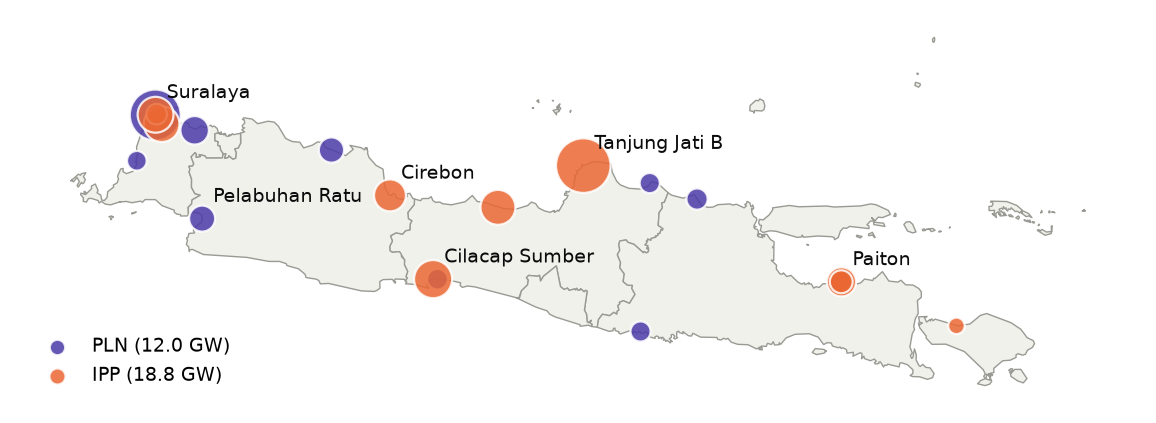
\includegraphics[width=\textwidth]{peta_pltu}
\caption{PLTU terhubung jaringan PLN di Jawa-Bali menurut pemilik (ukuran lingkaran sebanding kapasitas)}
\label{fig:peta}
\sumber{\textcite{D-GEM-GCPT}, batas wilayah \textcite{D-GEOBOUND}, diolah kelompok}
\end{figure}

\begin{table}[H]
\centering
\caption{PLTU jaringan PLN Jawa-Bali per provinsi}
\label{tab:pltu}
\small
\begin{tabular}{lrrrrrr}
\toprule
Provinsi & Unit & MW & IPP (MW) & PLN (MW) & Mt CO$_2$/tahun & Kematian/tahun \\
\midrule
Banten & 19 & 10.527 & 4.642 & 5.885 & 57,6 & 2.722 \\
Jawa Tengah & 15 & 10.090 & 8.800 & 1.290 & 52,4 & 2.610 \\
Jawa Timur & 12 & 6.155 & 3.365 & 2.790 & 36,3 & 1.592 \\
Jawa Barat & 8 & 3.624 & 1.584 & 2.040 & 19,9 & 1.676 \\
Bali & 3 & 426 & 426 & 0 & 2,7 & 110 \\
\midrule
Total & 57 & 30.822 & 18.817 & 12.005 & 168,9 & 8.710 \\
\bottomrule
\end{tabular}

\sumber{\textcite{D-GEM-GCPT} untuk kapasitas dan emisi. Kematian dini dihitung dari faktor rata-rata armada \textcite{P-CREA-IESR-2023}, kecuali Cirebon-1 yang memakai angka khusus CREA}
\end{table}

\subsection{Dampak Kesehatan}

CREA dan IESR memodelkan bahwa emisi PLTU batu bara pada 2022 menyebabkan sekitar 10.500 kematian dini dan biaya kesehatan US\$7,4 miliar \parencite{P-CREA-IESR-2023}. Jawa Barat adalah provinsi paling terdampak dengan lebih dari 4.000 kematian per tahun, disusul Banten (2.000) dan Jawa Tengah (1.700). Temuan ini sejalan dengan studi regional yang memproyeksikan kenaikan beban penyakit akibat ekspansi PLTU di Asia Tenggara \parencite{P-KOPLITZ-2017}.

Dampak tidak merata antar-PLTU. Di wilayah Jawa-Bali-Sumatra, CREA menempatkan Muara Karang, Lontar, Cirebon, Cirebon-2, dan Cilacap sebagai pembangkit dengan biaya kesehatan per kWh tertinggi karena dekat permukiman padat \parencite{P-CREA-IESR-2023}. Untuk Cirebon-1, CREA memperkirakan pensiun pada 2035 menghindari 6.370 kematian dan US\$4,4 miliar biaya kesehatan selama 2036-2042 \parencite{B-ECOBUSINESS-CIREBON}. Artinya, nilai kesehatan dari pensiun dini sangat bergantung pada PLTU mana yang dipilih.

\subsection{Pekerja dan Daerah}

Cirebon-1 mempekerjakan sekitar 300 orang, dan hanya 50 di antaranya berasal dari desa sekitar. CELIOS memperkirakan sedikitnya 14.000 pekerja terdampak bila Cirebon-1 dan Pelabuhan Ratu dipensiunkan, termasuk pekerja tidak langsung \parencite{B-ECOBUSINESS-CIREBON}. Sebaliknya, PLTS atap termasuk teknologi energi yang paling padat karya, sekitar 24,72 job-year per MW \parencite{P-CEEW-2017}. Transisi yang adil membutuhkan program alih keterampilan agar pekerja PLTU dapat berpindah ke sektor ini.

\subsection{Beban Rumah Tangga dan Fiskal}

Penjualan listrik PLN pada 2025 mencapai 317,69 TWh, dan 133,41 TWh di antaranya untuk rumah tangga \parencite{B-CNBC-SALES-2025}. Jawa-Bali menyerap 220,8 TWh atau 69,5\% dari penjualan nasional, dengan Jawa Barat sebagai pasar terbesar (63,5 TWh) \parencite{D-PLN-STAT-2025}. Subsidi listrik 2026 diusulkan Rp97,37-104,97 triliun untuk 44,88 juta pelanggan, dengan BPP Rp1.828-1.920 per kWh \parencite{B-KONTAN-SUBSIDI-2026}. Pelanggan 450 VA dan 900 VA bersubsidi membayar Rp415 dan Rp605 per kWh, sedangkan rumah tangga 1.300-2.200 VA membayar Rp1.444,70 per kWh \parencite{B-KOMPASTV-TARIF-2026}. Karena tarif ditetapkan di bawah BPP, setiap perubahan biaya PLN pada akhirnya berpindah ke APBN.

Tanpa net metering, PLTS atap rumah tangga menjadi kurang menarik karena konsumsi rumah tangga tinggi pada malam hari. IESR memperkirakan adopsi PLTS atap akan lebih banyak terjadi di sektor komersial dan industri \parencite{B-PVMAG-QUOTA,P-IESR-PERMEN2}.

\subsection{Dampak pada Keandalan Sistem}

Pada Februari 2024 daya mampu pasok sistem Jamali tercatat 37.364 MW dengan beban puncak tertinggi 28.077 MW \parencite{B-MATAHARI-2024}. Statistik PLN 2025 mencatat kapasitas terpasang Jawa 52.575 MW dan daya mampu 49.681 MW, termasuk pembangkit sewa dan IPP \parencite{D-PLN-STAT-2025}. Selisih ini terjadi karena daya mampu pasok hanya menghitung pembangkit yang siap dioperasikan, sehingga kajian ini memakai angka cadangan dari PLN UIP2B dan MKI. White Paper Masyarakat Ketenagalistrikan Indonesia (MKI) memperkirakan reserve margin turun dari 37,5\% pada 2025 ke bawah rentang aman 33-35\% pada 2027 jika beban tumbuh 4,45\% per tahun tanpa tambahan pembangkit yang cukup \parencite{B-PETROMINDO-RESERVE}. Kondisi ini penting: selama listrik berlebih, satu PLTU dapat dipensiunkan tanpa diganti, tetapi setelah jendela itu menutup, setiap PLTU yang pensiun membutuhkan pembangkit pengganti.
